%Made By Thomas Debelle
\documentclass{report}
\usepackage[a4paper, total={6in, 9in}]{geometry}
\usepackage[utf8]{inputenc}
\usepackage[francais]{babel}
\usepackage{graphicx}
\usepackage{graphics}
\usepackage[T1]{fontenc}
\usepackage{amsmath}
\usepackage{hyperref}
\usepackage{amssymb}
\usepackage{listings}
\usepackage{xcolor}
\usepackage{array}
\usepackage{float}
\usepackage{amsfonts}
\usepackage{fancyhdr}
\usepackage{titlesec}
\usepackage{xparse}
\usepackage{wrapfig}

\hypersetup{
    colorlinks=true,
    linkcolor=black,
    filecolor=magenta,
    urlcolor=cyan,
    pdftitle={Overleaf Example},
    pdfpagemode=FullScreen,
    }
\begin{document}


\begin{titlepage}
    \begin{figure}
        
\includegraphics[height = 2cm]{UCL_Logo.png}
        \label{fig:my_label}
    \end{figure}

    \hspace*{100cm}
    \centering
    \vspace*{7cm}

    {\Huge \textbf{Résumé de LELEC1370}}\\
    \vspace*{0.25cm}
    compilation du \today\\
    \vspace*{0.25cm}
    \Large{Thomas Debelle}\\

    \vspace*{9.5cm}
    {\Large Juin 2023}
\end{titlepage}


\tableofcontents
\newpage

\section*{Préface}

Bonjour à toi !\\

Cette synthèse recueille toutes les informations importantes données au cours, pendant les séances de tp et est amélioré grâce au note du Syllabus. Elle ne remplace pas le cours donc écoutez bien les conseils et potentielles astuces que les professeurs peuvent vous donner. Notre synthèse est plus une aide qui on l'espère vous sera à toutes et tous utiles.\\

Elle a été réalisée par toutes les personnes que tu vois mentionné. Si jamais cette synthèse a une faute, manque de précision, typo ou n'est pas à jour par rapport à la matière actuelle ou bien que tu veux simplement contribuer en y apportant ta connaissance ? Rien de plus simple ! Améliore la en te rendant \href{http://www.github.com/Tfloow/Q4_EPL}{ici} où tu trouveras toutes les infos pour mettre ce document à jour. (\textit{en plus tu auras ton nom en gros ici et sur la page du github})\\

Nous espérons que cette synthèse te sera utile d'une quelconque manière ! Bonne lecture et bonne étude.


\chapter{Cours 1}
\section{Les bases}

Tout d'abord, il existe 2 types de courant appelé \textbf{Direct Current} ou \textit{DC} et \textbf{Alternating Current} ou \textit{AC}. Le courant direct est continu tandis que le courant \textit{AC} varie dans le temps comme montré ci-contre.\\
\begin{figure}[H]
	\centering
	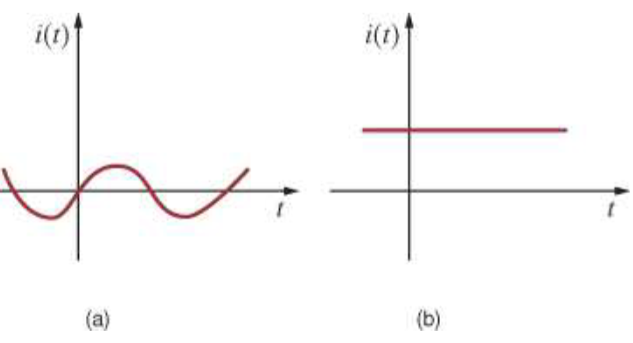
\includegraphics[width=.3\textwidth]{img/ACDC.png}
	\caption{Gauche: courant AC \quad Droite: courant DC}
\end{figure}
La tension vaut la variation d'énergie selon la charge ou autrement dit: 
\begin{equation}
v = \frac{dw}{dq}
\end{equation}
La puissance vaut la tension par le courant ou:
\begin{equation} \label{eqn:p}
p = vi = \frac{dw}{dq}\frac{dq}{dt}
\end{equation}
Finalement, l'énergie est une différence de puissance en fonction du temps:
\begin{equation}
\Delta w = \int_{t_1}^{t_2}p dt = \int_{t_1}^{t_2} vi dt
\end{equation}
Quelques conventions:
\begin{itemize}
\item Source de tension nulle = court circuit
\item Source de courant nulle = circuit ouvert
\item Le sens du courant "rentre" dans la borne + d'un générateur de tension.
\end{itemize}
\subsubsection{Puissance dissipée}
Pour connaitre la puissance dissipée dans une résistance, on utilise d'abord la formule fondamentale d'une résistance:
\begin{equation}
v(t) = R i(t)
\end{equation}
Ainsi, en utilisant \ref{eqn:p} on trouve:
\begin{equation}
p(t) = vi(t) = \frac{v^2(t)}{R} = Ri^2(t)
\end{equation}

\subsubsection{Loi des noeuds de Kirchoff}
La somme des courants de tous les noeuds a pour résultat 0. Autrement dit, tout courant qui apparait disparait quelque part.

\subsubsection{Loi des mailles de Kirchoff}
Dans un circuit électrique, on peut dessiner des \textit{mailles} ou des sortes de carrés. En tournant dans un sens, on fait la somme des tensions (\textit{faire attention au sens des tensions}) on obtient une somme nulle.

\subsubsection{Sources multiples - Diviseur de tension}
On peut simplifier un circuit et sommer des sources de tension en additionnant leur tension. On utilise également la règle des diviseurs de tension pour les résistances:
\begin{equation}
\begin{cases}
\parallel \rightarrow R_{new} = \frac{1}{\frac{1}{R_1}+\frac{1}{R_2}}\\
\text{série} \rightarrow R_{new} = R_1 + R_2
\end{cases}
\end{equation}

\subsubsection{Mise en parallèle et sources multiples}
Les sources de courant en parallèle peuvent être sommé pour les simplifier et n'en avoir qu'une seule source de courant.

\subsubsection{Équivalent Thévenin Norton}
On peut simplifier une alimentation d'un circuit via les circuits de Thévenin et Norton. Thévenin est composé d'une source de tension et d'une résistance en série tandis que Norton a une source de courant et une résistance en parallèle.\\
Les choses importantes à noter sont:
\begin{equation}
\begin{cases}
R_{Th} = R_{No}\\
I_{sc} = \frac{V_{R}}{R_{Th}}\\
v_{oc} = R_{Th}i_{sc}
\end{cases}
\end{equation}
 
\begin{figure}[H]
\centering
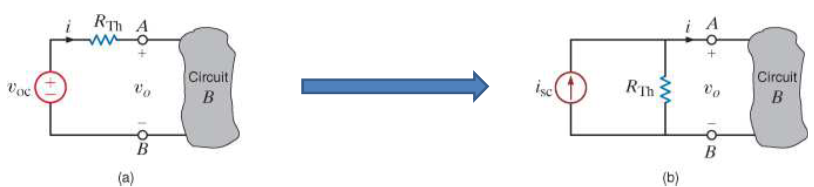
\includegraphics[width = 10cm]{img/ThNo.png}
\caption{Illustration du passage de Thévenin à Norton}
\end{figure}

\chapter{Cours 2}
\subsubsection{Le quadripole}

\end{document}


